\documentclass[10pt,letterpaper]{article}
\usepackage[top=1in,bottom=1in,left=1in,right=1in]{geometry}
\usepackage{datetime}
\usepackage{natbib}      % http://merkel.zoneo.net/Latex/natbib.php
\usepackage{palatino}
\usepackage{verbatim}
\usepackage[normalem]{ulem}
\bibpunct{(}{)}{;}{a}{,}{,}

\usepackage{array}

\usepackage{chngpage}
\usepackage{stmaryrd}
\usepackage{amssymb}
\usepackage{amsmath}
\usepackage{graphicx}
\usepackage{lscape}
\usepackage{subfigure}
\usepackage[usenames,dvipsnames]{color}
\definecolor{myblue}{rgb}{0,0.1,0.6}
\definecolor{mygreen}{rgb}{0,0.3,0.1}
\usepackage[colorlinks=true,linkcolor=black,citecolor=mygreen,urlcolor=myblue]{hyperref}

\newcommand{\bocomment}[1]{\textcolor{Bittersweet}{BO says: #1}}

\newcommand{\ignore}[1]{}
\newcommand{\transpose}{^\mathsf{T}}
\newcommand{\inner}[1]{\langle #1 \rangle} 
\newcommand{\smallsec}[1]{\noindent \textbf{#1\ }}
\newcommand{\cmd}[1] {{\color{blue}\texttt{#1}}}

\newcommand{\solution}[1]{{\color{myblue} \emph{[Solution:} 

#1 

\emph{End solution]}}}
\newcommand{\solutionnote}[1]{{\color{myblue} \emph{[Note:}

#1 

\emph{End note]}}}
\newcommand{\points}[1]{{\color{mygreen}\emph{[#1]\ \ }}}

\newcommand{\aone}{\diamondsuit}
\newcommand{\atwo}{\heartsuit}
\newcommand{\bone}{\triangle}
\newcommand{\btwo}{\Box}
\newcommand{\myand}{\ \land\ }
\newcommand{\myor}{\ \lor\ }
\newcommand{\mynot}{\lnot}

\title{
	Mini-project 2 \\
	\Large{COMPSCI 370, Spring 2021, UMass Amherst} \\
	\Large{Instructor: Subhransu Maji} \\
	\Large{TAs: Chenyun Wu, Jong-Chyi Su}
}


\settimeformat{ampmtime}
\date{}
\begin{document}
\maketitle

\renewcommand\thesubsection{\thesection.\alph{subsection}}
\section*{Guidelines}
\paragraph{Submission.} Submit a \emph{single pdf} file via
Gradescope that includes your solutions, figures, and code. The latex
source file for the homework is provided in case you want to modify it
to produce your report. However, you are welcome to use other
typesetting software as long as the final output is a pdf.
For readability you may attach the code printouts at the end of the
solutions within the same pdf.
Similarly figures enable easy comparision of various approaches.
Poorly written or formatted reports will make it harder for us to
evaluate it and may lead to a deduction of credit.


\paragraph{Late policy.}
\begin{itemize}
\item You can use 7 late days, with up to 3 late days per assignment.
\item Once you have used all 7 late days, penalty is 25\% for each additional late day.
\item We will use your latest submission for grading and for calculating your late day usage.
\item There is no bonus if you don't use late days at all.
\end{itemize}


\paragraph{Plagiarism.}
We expect the students not to copy, refer to, or look at the solutions
in preparing their answers. We expect students to want to learn and
not google for answers. See the Universities' guidelines on academic
honesty (\url{https://www.umass.edu/honesty}).
Finally, we also ask you to not post the solutions online as the
problem sets might be used in future.


\paragraph{Collaboration.} The homework must be done individually,
except where otherwise noted in the assignments. 'Individually' means
each student must hand in their own answers, and each student must
write their own code in the programming part of the assignment. It is
acceptable, however, for students to collaborate in figuring out
answers and helping each other solve the problems, for example within
a study group.
We will be assuming that you will be taking the responsibility to make
sure you personally understand the solution to any work arising from
such a collaboration.


\paragraph{Python requirements.}
Our code is tested on Python 3.
The Python code depends on external
packages such as \cmd{scipy}, \cmd{numpy}, and \cmd{scikit-image}.
Take a look at the resources posted on the course page to set up the
appropriate programming environment and tutorial on basic concepts.


\paragraph{Using other programming languages.}
While we have made the starter code available in Python, 
feel free to implement the homework from scratch using your favorite
programming language. For example you are welcome to use Matlab, C, Java,
Octave or Julia, with the caveat that we may be able help you with
debugging.







\newpage



\section{Aligning Prokudin-Gorskii images [25 points]} 
Sergei Mikhailovich Prokudin-Gorskii was a Russian chemist and photographer ahead of his time. 
Even though color photography was not yet invented, he had the brilliant idea to capture color pictures by simply taking pictures of a scene, with a red, green and blue filter.
There was no way of printing these back in the day, so he envisioned complex display devices to show these. However these were never made during his lifetime, but his pictures survived. 
In this homework you will reconstruct a color image taken from a collection of images from a photographic survey of the Russian Empire he conducted for Tsar Nicholas II. 
Figure 1 illustrates the idea.

\begin{figure}[h]
\centering
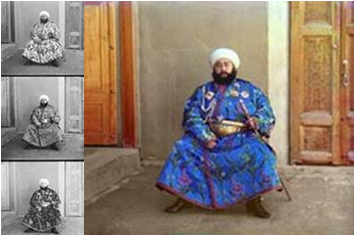
\includegraphics[width=0.65\linewidth]{example-Prokudin-Gorskii.png}
\caption{Example image from the Prokudin-Gorskii collection. On the left are the three images captured individually. On the right is a reconstructed color photograph. Note the colors are in B, G, R order from the top to bottom (and not R, G, B)!}
\end{figure}

Recall that color images are represented digitally as RGB color channels. Thus if we stack the three channels in the right order then the color image will be displayed. 
Alas, since the three pictures weren't taken from the same position due to the camera motion in between shots, the images are likely to be misaligned. 
The key to obtain a crisp color image is to align the three photographs.
For this homework you will assume that the motion is a pure translation.

Your strategy for alignment will be to search over a range of displacements in X and Y directions for each channel.
The simplest way is to keep one channel fixed say R, and align the G, B channels to it by searching over displacements in the range [-15, 15] both horizontally and vertically and pick the displacement that maximizes similarity between the channels.
One such measure is the angle between vectors of pixels in each channel. Recall that the angle between two vectors $a$ and $b$ given by
$$
	\cos \theta = \frac{a^Tb} {||a||\cdot||b||},
$$
where $||a|| = \sqrt{a^Ta}$ denotes the norm (or length) of a vector. 

\subsection{Code}
Download the \cmd{p2-release.zip} from the moodle page. Move them to your homework directory and extract the files. The code, data, and latex source files are in the \cmd{p2-release/code}, \cmd{p2-release/data}, and \cmd{p2-release/latex} folders respectively.

Before you start aligning the Prokudin-Gorskii images (in $\cmd{data/prokudin-gorskii}$), you will test your code on randomly shifted synthetic images. Your code should correctly discover the inverse of the shift.

Run \cmd{evalAlignment} inside the code directory. This should produce the following output. Note the actual 'gt shift' might be different since it is randomly generated.
\begin{verbatim}
    Evaluating alignment ..
    1 balloon.jpeg
	   gt shift: ( 1,11) ( 4, 5)
	 pred shift: ( 0, 0) ( 0, 0)
    2 cat.jpg
	   gt shift: (-5, 5) (-6,-2)
	 pred shift: ( 0, 0) ( 0, 0)
     ...
\end{verbatim}
    
The code loads a set of images, randomly shifts the color channels and provides them as input to \cmd{alignChannels}. Your goal is to implement this function. A correct implementation should obtain the shifts that is the negative of the ground-truth shifts, i.e. the following output:

\begin{verbatim}
    Evaluating alignment ..
    1 balloon.jpeg
	   gt shift: ( 13, 11)  ( 4, 5)
	 pred shift: (-13,-11)  (-4,-5)
    2 cat.jpg
	   gt shift: (-5, 5) (-6,-2)
	 pred shift: ( 5,-5) ( 6, 2)
     ...
\end{verbatim}

Once you are done with that, run \cmd{alignProkudin}. This will call your function to align images from the Prokudin-Gorskii collection. The output is saved to the \cmd{outDir}. Note that if this directory does not exist, you will have to create it first. 
In your report show all the aligned images as well as the shifts that were computed by your algorithm.

Tips: Look at functions \cmd{np.roll} and \cmd{np.pad} in Python to deal with shifting images.
% \cmd{circshift()} and \cmd{padarray()} to deal with shifting images in Matlab.


\subsection{What to submit?}
To get full credit for this part you have to 
\begin{itemize}
\item include your implementation of \cmd{alignChannels},
\item verify that the \cmd{evalAlignment} correctly recovers the color image and shifts for the toy example, 
\item include the aligned color images from the output of \cmd{alignProkudin},
\emph{including} the computed shift vectors for each image.
\end{itemize}

\subsection{Extra credit}
Here are some ideas for extra credit.
\begin{itemize}
\item Shifting images can cause ugly boundary artifacts. Come up with of a way of avoiding this.
\item Searching over displacements can be slow. Think of a way of aligning them faster in a coarse-to-fine manner. For example, you may align the channels by resizing them to half the size and then refining the estimate. This can be done by multiple calls to your \cmd{alignChannels()} function.
\end{itemize}
If you do these, or any other, for extra credit make sure to include the code, description and any other details that you think are relevant for grading such as figures, run-time analysis, etc.

\section{Color image demosaicing [35 points]}
Recall that in digital cameras the red, blue, and green sensors are interlaced in the Bayer pattern (Figure~\ref{fig:bayer}) and missing values are interpolated to obtain a full color image. 
For this part you will implement the \emph{nearest-neighbor} interpolation algorithm. 
The input to the algorithm is a single image \cmd{im}, a NxM array of numbers between 0 and 1. 
These are measurements in the format shown in Figure~\ref{fig:bayer}, i.e., top left \cmd{im(1,1)} is red, \cmd{im(1,2)} is green, \cmd{im(2,1)} is green, \cmd{im(2,2)} is blue, etc. Your goal is to create a single color image C from these measurements. Note that in Python/NumPy, those coordinates are expressed as \cmd{im[0,0]}, \cmd{im[0,1]}, \cmd{im[1,0]}, \cmd{im[1,1]}.
\begin{figure}[h]
\centering
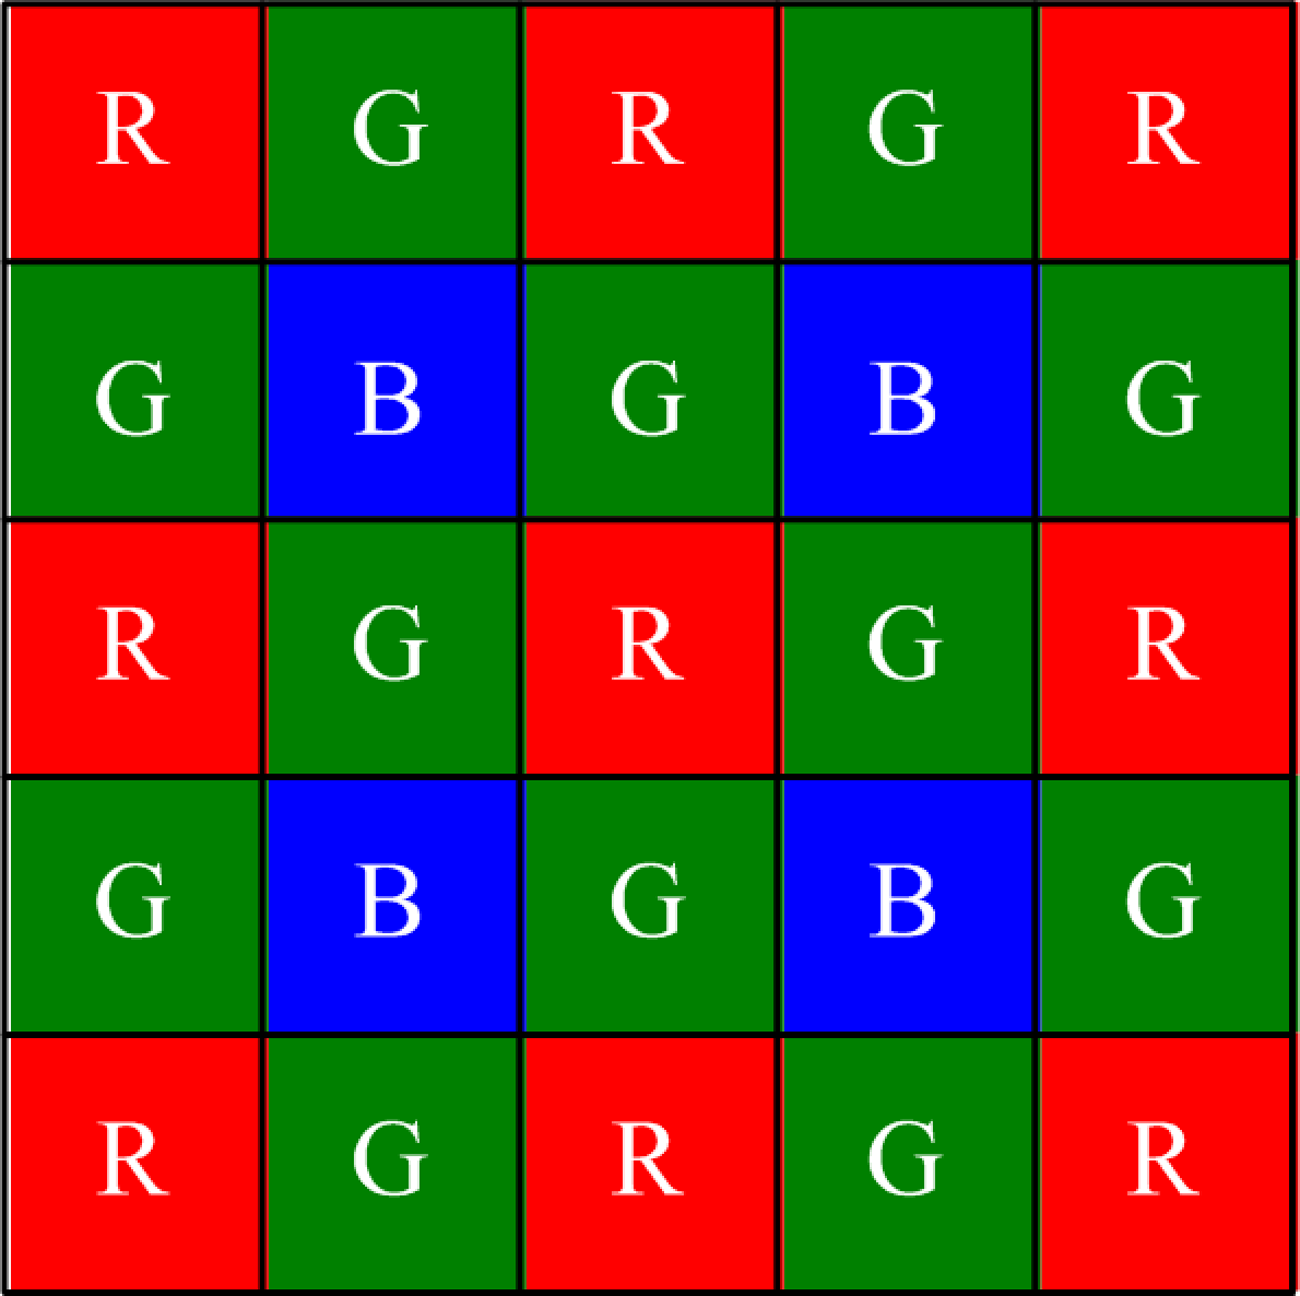
\includegraphics[width=0.2\linewidth]{bayer-pattern.png}
\caption{\label{fig:bayer} Bayer pattern}
\end{figure}

Your entry point for this part of the homework in \cmd{evalDemosaic}. The code loads images from the data directory (in $\cmd{data/demosaic}$), artificially mosaics them (\cmd{mosaicImage} file), and provides them as input to the demosaicing algorithm (\cmd{demosaicImage} file). By comparing the result with the input we can also measure an error computed as the distance between the reconstructed image and the true image in pixel space. This is what the algorithm reports. Once you have implemented the \cmd{mosaicImage} function run the \cmd{evalDemosaic} and you should see the output below.

Only the \cmd{demosaicImage(im, 'baseline')} is implemented in the provided code. The baseline simply replaces all the missing values for a channel with the average value of that channel. 
Your goal is to implement the nearest-neighbor interpolation approach (\cmd{demosaicImage(im, 'nn')}), which should obtain significantly lower errors.
Right now it simply calls the baseline algorithm hence the two methods produce identical results.

\begin{verbatim}
--------------------------------------------
# 	 image             baseline   nn
--------------------------------------------
1 	 balloon.jpeg      0.179239 	 0.179239 
2 	 cat.jpg           0.099966 	 0.099966 
3 	 ip.jpg            0.231587 	 0.231587 
4 	 puppy.jpg         0.094093 	 0.094093 
5 	 squirrel.jpg      0.121964 	 0.121964 
6 	 pencils.jpg 	     0.183101 	 0.183101 
7 	 house.png         0.117667 	 0.117667 
8 	 light.png         0.097868 	 0.097868 
9 	 sails.png         0.074946 	 0.074946 
10  tree.jpeg         0.167812 	 0.167812 
--------------------------------------------
 	  average           0.136824 	 0.136824 
--------------------------------------------
\end{verbatim}
You will implement the two functions:
\begin{enumerate}
\item \points{10 points} Implement \cmd{mosaicImage(im)}. This function takes an image \cmd{im} with three color channels and returns \cmd{mosim} that has a single channel where the red, green, and blue pixels are copied according to the Bayer pattern shown in the figure. This function simulates the sensor in the digital camera.

\item \points{20 points} Implement \cmd{demosaicImage(im, 'nn')}. This function takes the demosaiced image and reconstructs the three color channels. The `nn' option stands for \emph{nearest-neighbor} interpolation, i.e. you simply copy the value of the nearest available pixel. For example, each missing green pixel can copy the value  of the green pixel to its left (note that this doesn't work on the left boundary where you can copy from the top or bottom). This very simple method should produce reasonable results and substantially lower errors (around $0.025$ average error) when you run \cmd{evalDemosaic}.

\item \points{5 points} The nearest neighbor interpolation relies on smoothness of natural images, i.e., nearly pixels are roughly of the same value. Create a plot where the value of a pixel for the red channel is plotted against the value of the pixel to its right for the red channel. Similarly create plots for the green and blue channels. 
Use the image \cmd{data/demosaic/puppy.jpg} for this plot. What do you observe?




\end{enumerate}

\subsection{What to submit?}
To get full credit for this part you have to 
\begin{itemize}
\item include your implementation of \cmd{mosaicImage} and \cmd{demosaicImage},
\item include the output of \cmd{evalDemosaic}.
\item include the three plots for the \cmd{puppy.jpg} image.
\end{itemize}

\subsection{Extra credit}
There are numerous other approaches for interpolation which you can read on the internet. You can use the ideas but do not copy the code (we can easily detect if you have simply copied the code from the web). You can implement this as other options \cmd{demosaicImage(im, `yourmethod')} and include the list of options in the \cmd{evalDemosaic} code. It is possible to get errors as low as $0.017$ without too much effort.

\section{Submission and rubric}
\begin{itemize}
\item Follow the outline on Gradescope for your submission. This will make it easier for us to grade different parts of your solutions.
\item A fraction of the points for each coding assignment will be for readability and efficiency of your code. Thus it is important to properly document parts of the code you implemented.
\end{itemize}





\end{document}
